\documentclass[a4paper]{article}
% \usepackage[a4paper]{geometry}
\usepackage{fullpage}
\usepackage{times}
\usepackage{epsfig,endnotes}
\usepackage{algorithm}
\usepackage{threeparttable}
\usepackage{algorithmic}
\usepackage{amssymb,amsmath}
\usepackage{color}
\usepackage{comment}
\usepackage{multirow}
\usepackage{graphicx,subfigure}
\usepackage{url}
\usepackage{alltt}
\usepackage{listings}
\usepackage[T1]{fontenc}
\usepackage{kantlipsum}
\usepackage[usenames,dvipsnames]{xcolor}
\usepackage[breakable, theorems, skins]{tcolorbox}
\tcbset{enhanced}
\usepackage[normalem]{ulem}
\DeclareGraphicsExtensions{.pdf,.png,.jpg}
\lstset{basicstyle=\ttfamily\small, language=C, breaklines=true}
\definecolor{lightblue}{cmyk}{1, 0.50, 0, 0}
\definecolor{darkblue}{rgb}{0.0, 0.2, 0.5}
\DeclareRobustCommand{\mybox}[2][gray!20]{%
\begin{tcolorbox}[   %% Adjust the following parameters at will.
        breakable,
        left=0pt,
        right=0pt,
        top=0pt,
        bottom=0pt,
        colback=#1,
        colframe=#1,
        width=\dimexpr\textwidth\relax,
        enlarge left by=0mm,
        boxsep=5pt,
        arc=0pt,outer arc=0pt,
        ]
        #2
\end{tcolorbox}
}


\begin{document}

\begin{flushleft}
{\Large \textbf{C0}
\line(1, 0){450}}
\end{flushleft}

{\section{Introduction}}

C0 is grammatically similar to the C language and will be immediately familiar to C, C++ and Java programmers. It is a procedure-oriented language with linguistic support for massive parallelism on a modern compute cluster.

{\subsection{Simple example}}

Here we have a parallel version of vector addition it in C0.

{\color{blue}{\lstinputlisting[language=C]{examples/add.c}}}

The above program adds two vectors of length 10000 with 100 runners, each runner adds up 100 elements. A runner is a separate execution of code which is similar to threads.

{\subsection{Program structure}}

The four key concepts in C0 are programs, types, variables and functions. A program consists of one or more source files. Each source file defines some types or functions. The program must have a function named \textbf{\texttt{main}} with no parameter or return value. The program starts from the \textbf{\texttt{main}} function.

{\subsection{Keywords}}

\begin{table}[htbp]
\centering
\caption{C0 key words}
\begin{tablenotes}
\small
\centering
\item The supported key words currently.
\end{tablenotes}
\begin{tabular}{|l|l|l|l|}
\hline
abort & break & goto & if\\
\hline
continue & else & long & commit \\
\hline
double & commitd & return & unsigned\\
\hline
char & signed & runner & void\\
\hline
while & for & do & watching\\
\hline
in & abortd & standalone & \\
\hline
\end{tabular}
\label{table:key-words}
\end{table}

The following keywords are to be supported:
\textbf{\texttt{default}}
,\textbf{\texttt{static}}
,\textbf{\texttt{sizeof}}
,\textbf{\texttt{register}}
,\textbf{\texttt{short}}
,\textbf{\texttt{auto}}
,\textbf{\texttt{struct}}
,\textbf{\texttt{bool}}
,\textbf{\texttt{int}}
,\textbf{\texttt{switch}}
,\textbf{\texttt{true}}
,\textbf{\texttt{const}}
,\textbf{\texttt{float}}
,\textbf{\texttt{case}}
,\textbf{\texttt{enum}}
,\textbf{\texttt{false}}
,\textbf{\texttt{extern}}
,\textbf{\texttt{volatile}}

{\section{Types}}

There are several types in C0: simple types, struct types, union types, function types, void type, pointer types, array types, and array segments.

{\subsection{Simple types}}

Table~\ref{table:c0-types} shows the simple types supported (Or would be supported) in C0.

\begin{table}[htbp]
\centering
\caption{Simple types in C0}
\begin{tablenotes}
\small
\centering
\item Note: The key words in yellow are not supported currently.
\end{tablenotes}
\begin{tabular}{|l|l|l|l|}
\hline
category & bits & type & range/precision\\
\hline
\colorbox{yellow}{boolean} & \colorbox{yellow}{32} & \colorbox{yellow}{bool} & \colorbox{yellow}{true or false}\\
\hline
\multirow{4}{*}{signed integral} & 8 & char & -128...127\\\cline{2-4}
 & \colorbox{yellow}{16} & \colorbox{yellow}{-} & \colorbox{yellow}{-32,768...32,767}\\\cline{2-4}
 & \colorbox{yellow}{32} & \colorbox{yellow}{int} & \colorbox{yellow}{-2,147,483,648...2,147,483,647}\\\cline{2-4}
 & 64 & long & -9,223,372,036,854,775,808...9,223,372,036,854,775,807\\\cline{2-4} \hline
\multirow{4}{*}{unsigned integral} & 8 & unsigned char & 0...255\\\cline{2-4}
 & \colorbox{yellow}{16} & \colorbox{yellow}{-} & \colorbox{yellow}{0...65,535}\\\cline{2-4}
 & \colorbox{yellow}{32} & \colorbox{yellow}{unsigned int} & \colorbox{yellow}{0...4,294,967,295}\\\cline{2-4}
 & 64 & unsigned long & 0...18,446,744,073,709,551,615\\\cline{2-4} \hline
\multirow{2}{*}{floating point} & \colorbox{yellow}{32} & \colorbox{yellow}{float} & \colorbox{yellow}{1.5 * 10 - 45 to 3.4 * 1038, 7 - digit precision}\\\cline{2-4}
 & 64 & double & 5.0 * 10 - 324 to 1.7 * 10308, 15 - digit precision\\\cline{2-4} \hline
\end{tabular}
\label{table:c0-types}
\end{table}

{\subsection{Struct/Union types (not supported yet)}}

Structure types are user defined types which contains other types (including other structure types).  The struct keyword is used to define a structure type. Each element of a structure is called field. Each field in a structure has its own storage space.

{\color{blue}{\lstinputlisting[language=C]{examples/struct.c}}}

The union types are similar to structure types. But the field in union shares the common storage space, so at most one field contains a meaningful value at any given time.

{\subsection{Function types}}
In the program, you cannot directly define variables of function types. But you can define functions who has a function type, or define a function pointer to a specified function type.
A function type describes the function prototype, including the types of parameters and the type of return value.

{\subsection{Void type}}
Void type is a special type which means "no type", it can only be used for the return type of function, which means the function does not return any value, or used for defining a pointer which can points to any kind of values.

{\subsection{Pointer types}}
A variable of pointer type stores the address of the underlying type. We can access the value stored in the memory location which the pointer points to. This operation is called dereferencing a pointer. However, a pointer whose underlying type is void type cannot be dereferenced.

{\subsection{Array types}}
An array is a data structure that contains a number of variables that are accessed through computed indices. The variables contained in an array, also called the elements of the array, are all of the same type, and this type is called the element type of the array. We use array[index] to access the elements of an array. The indices of the elements of an array range from 0 to Length - 1.

{\subsection{Array segment}}
An array segment is logically same as an array (or a pointer). However, it restricts the access of elements to a specified range. The array segment is represented as array[start,,end], the start is inclusive and end is exclusive.

{\subsection{Standalone}}
standalone is a special keyword of C0. It is for global variables which are in the Shared Region (SR). When a global variable is standalone, it always monopolizes one or many memory pages. The main purpose of using standalone is to reduce commit conflict among different global variables, since the basic unit of memory space management is a page.

{\color{blue}{\lstinputlisting[language=C]{examples/standalone.c}}}

For the above example, if runner A modify a and runner B modify b, there will be no commit conflict.

{\section{Expressions and Statements}}

{\subsection{Expressions}}

Expressions are constructed from operands and operators. The operators of an expression indicate which operations to apply to the operands. Examples of operators include +, -, *, /. Examples of operands include literals, fields, local variables, and expressions.

When an expression contains multiple operators, the precedence of the operators controls the order in which the individual operators are evaluated. For example, the expression x + y * z is evaluated as x + (y * z) because the * operator has higher precedence than the + operator.

\begin{table}[htbp]
\centering
\caption{Operators in C0}
\begin{tablenotes}
\centering
\small
\item Note: The key words in yellow are not supported currently.
\end{tablenotes}
\begin{tabular}{|l|l|l|}
\hline
Category & Expression & Description\\
\hline
\multirow{6}{*}{Primary} & x.m & Field access\\\cline{2-3}
 & x(...) & Method invocation\\\cline{2-3}
 & x[...] & Array or array segment access\\\cline{2-3}
 & \colorbox{yellow}{x++} & Post-increment\\\cline{2-3}
 & \colorbox{yellow}{x\texttt{--}} & Post-decrement\\\cline{2-3}
 & x-\texttt{>}y & Pointer\\ \hline
\multirow{9}{*}{Unary} & *x & Dereference\\\cline{2-3}
 & \&x & Referencing the address\\\cline{2-3}
 & +x & Identity\\\cline{2-3}
 & -x & Negation\\\cline{2-3}
 & \colorbox{yellow}{!x} & Logical negation\\\cline{2-3}
 & \colorbox{yellow}{~x} & Bitwise negation\\\cline{2-3}
 & \colorbox{yellow}{++x} & Pre-increment\\\cline{2-3}
 & \colorbox{yellow}{\texttt{--}x} & Pre-decrement\\\cline{2-3}
 & (T)x & Explicitly convert x to type T\\ \hline
\multirow{3}{*}{Multiplicative} & x * y & Multiplication\\\cline{2-3}
 & x / y & Division\\\cline{2-3}
 & \colorbox{yellow}{x \% y} & \colorbox{yellow}{Remainder}\\ \hline
\multirow{2}{*}{Additive} & x + y & Addition\\\cline{2-3}
 & x - y & Subtraction\\ \hline
\multirow{2}{*}{\colorbox{yellow}{Shift}} & \colorbox{yellow}{x \texttt{<<} y} & \colorbox{yellow}{Shift left}\\\cline{2-3}
 & \colorbox{yellow}{x \texttt{>>} y} & \colorbox{yellow}{Shift right}\\ \hline
\multirow{4}{*}{Relational} & x \texttt{<} y & Less than\\\cline{2-3}
 & x \texttt{>} y & Greater than\\\cline{2-3}
 & x \texttt{<=} y & Less than or equal\\\cline{2-3}
 & x \texttt{>=} y & Greater than or equal\\ \hline
\multirow{2}{*}{Equality} & x == y & Equal\\\cline{2-3}
 & x != y & Not equal\\ \hline
Bitwise AND & x \& y & Integer bitwise AND\\ \hline
Bitwise XOR & x {\char`\^} y & Integer bitwise XOR\\ \hline
Bitwise OR & x \texttt{|} y & Integer bitwise OR\\ \hline
Logical AND & \colorbox{yellow}{x \&\& y} & Boolean logical AND\\ \hline
Logical OR & \colorbox{yellow}{x \texttt{||} y} & Boolean logical OR\\ \hline
Conditional & \colorbox{yellow}{x ? y : z} & Evaluates y if x is true, z if x is false\\ \hline
\multirow{2}{*}{Assignment} & x = y & Assignment\\\cline{2-3}
 & {\colorbox{yellow}{x op= y}} & {Compound assignment; supported operators are \colorbox{yellow}{*=  /= \%= +=  -=  \texttt{<<=}  \texttt{>>=}  \&=  {\char`\^}=  \texttt{|=}}}\\ \hline
\end{tabular}
\label{table:c0-operators}
\end{table}

Table~\ref{table:c0-operators} summarizes C0 operators, listing the operator categories in order of precedence from highest to lowest. Operators in the same category have equal precedence.

{\subsection{Statements}}

The actions of a program are expressed using statements.
A block permits multiple statements to be written in contexts where a single statement is allowed. A block consists of a list of statements written between the delimiters { and }.
Declaration statements are used to declare local variables and constants.
Expression statements are used to evaluate expressions. Expressions that can be used as statements include method invocations, assignments using = and the compound assignment operators, and increment and decrement operations using the ++ (Not supported yet) and -- (Not supported yet) operators.
Selection statements are used to select one of a number of possible statements for execution based on the value of some expressions. In this group are the if and switch statements.
Iteration statements are used to repeatedly execute an embedded statement. In this group are the while, do, and for statements.
Jump statements are used to transfer control. In this group are the break, continue, goto, and return statements.


{\section{Task and depending task}}

% {\subsection{Create a task}}

Defining a task is just the same as defining a function. Actually any function satisfying the necessary constraints (will be mentioned later) can be started as a task. A same function can either be directly invoked or be started as a new task.

The function that can become a task must have the prototype with the following constraints

\begin{itemize}
	\item It has no return type (with return type void)
	\item The parameters can only be either 1) simple types, or 3) array segments, or 3) structure types whose fields meet the constraints of 1) or 3).
\end{itemize}

The above constraints ensure that the input parameters to a new task will not reference external memory locations not in the range of the parameters. The use of array segments constraints the use of pointers so the runtime can create the snapshots efficiently.

{\subsection{Creating task instances}}

The syntax of creating a task is the same as invoking a function, plus the keyword \textbf{\textit{runner}}. Note that the task will only start to execute after current task exits.

Example (quick sort):

{\color{blue}{\lstinputlisting[language=C]{examples/sort.c}}}

{\subsection{Depending tasks}}

Depending tasks are tasks with additional startup conditions. Specifically, it will start after the parent task commits successfully and the specified memory location has been modified since the creation of the depending task.

Defining a depending task is similar to define a normal task.
To create a depending task, we also use task keywords, with additional parameters to specify the memory location to watch. The depending task will get executed if the content of the memory has changed. The parameter can either be the pointer to a simple type or structure type, or an array segment.

{{{\lstinputlisting[language=C]{examples/watcher.c}}}}

\paragraph{Difference between ``commit'' and ``commitd'', ``abort'' and ``abortd''.} ``commitd'' and ``abortd'' are for depending tasks only. Normal tasks only use ``commit'' and ``abort''.

For depending tasks:

\begin{enumerate}
\item When you create a depending task, you create a depending task type which can be considered as a ``task template''.
\item The depending task type watches the commits to the watched memory ranges.
\item When a depending task type is activated, a depending task instance, which can be considered as a normal task, is created. That is, the depending task type keeps watching the memory range changes after it is activated.
\item If there is a depending task instance in the task queue waiting to be scheduled, a commit to the depending task's depending ranges will not activate the depending task and create an instance any more.
\item The ``commit'' and ``abort'' have effect on the depending task instance only.
\item The ``commitd'' and ``abortd'' will commit/abort and delete the depending task type upon success.
\end{enumerate}

This way, it is ensured that after each commits to the watched ranges by a depending task, at least one depending task instance is created. Hence, no changes are missed by the depending task before it deletes itself by ``commitd'' or ``abortd'', and many changes may be ``aggregatively'' checked by a depending task instance for avoiding creating too many depending task instances that will abort and improving the efficiency.

{{\subsection{Creating tasks in another space}}}

The addressable memory in i0 contains many ``spaces''. Each space has a space specifier and the offset ranges for all spaces are the same. By default, the task statement creates tasks in the same space as the parent task. The space can be specified by the in clause of the task statement.

For example, to create a qsort task in space SPACE1:

{\color{blue}{\lstinputlisting[language=C]{examples/task.c}}}

The AMR as discussed in Section~\ref{mem-layout} is used for data communication across spaces since a task can only run inside of one space. The changes to memory ranges in AMR will activates all depending tasks in any space that watch the ranges.

{\section{Runtime Environment}}

\subsection{Memory Layout}
\label{mem-layout}

Each task runs in one space of the many spaces supported. The aliased memory region (AMR) is accessible from all spaces and can be used to share data across spaces. Fig.~\ref{fig:c0-spaces} illustrates the spaces.

\begin{figure}[htbp]
\begin{center}
  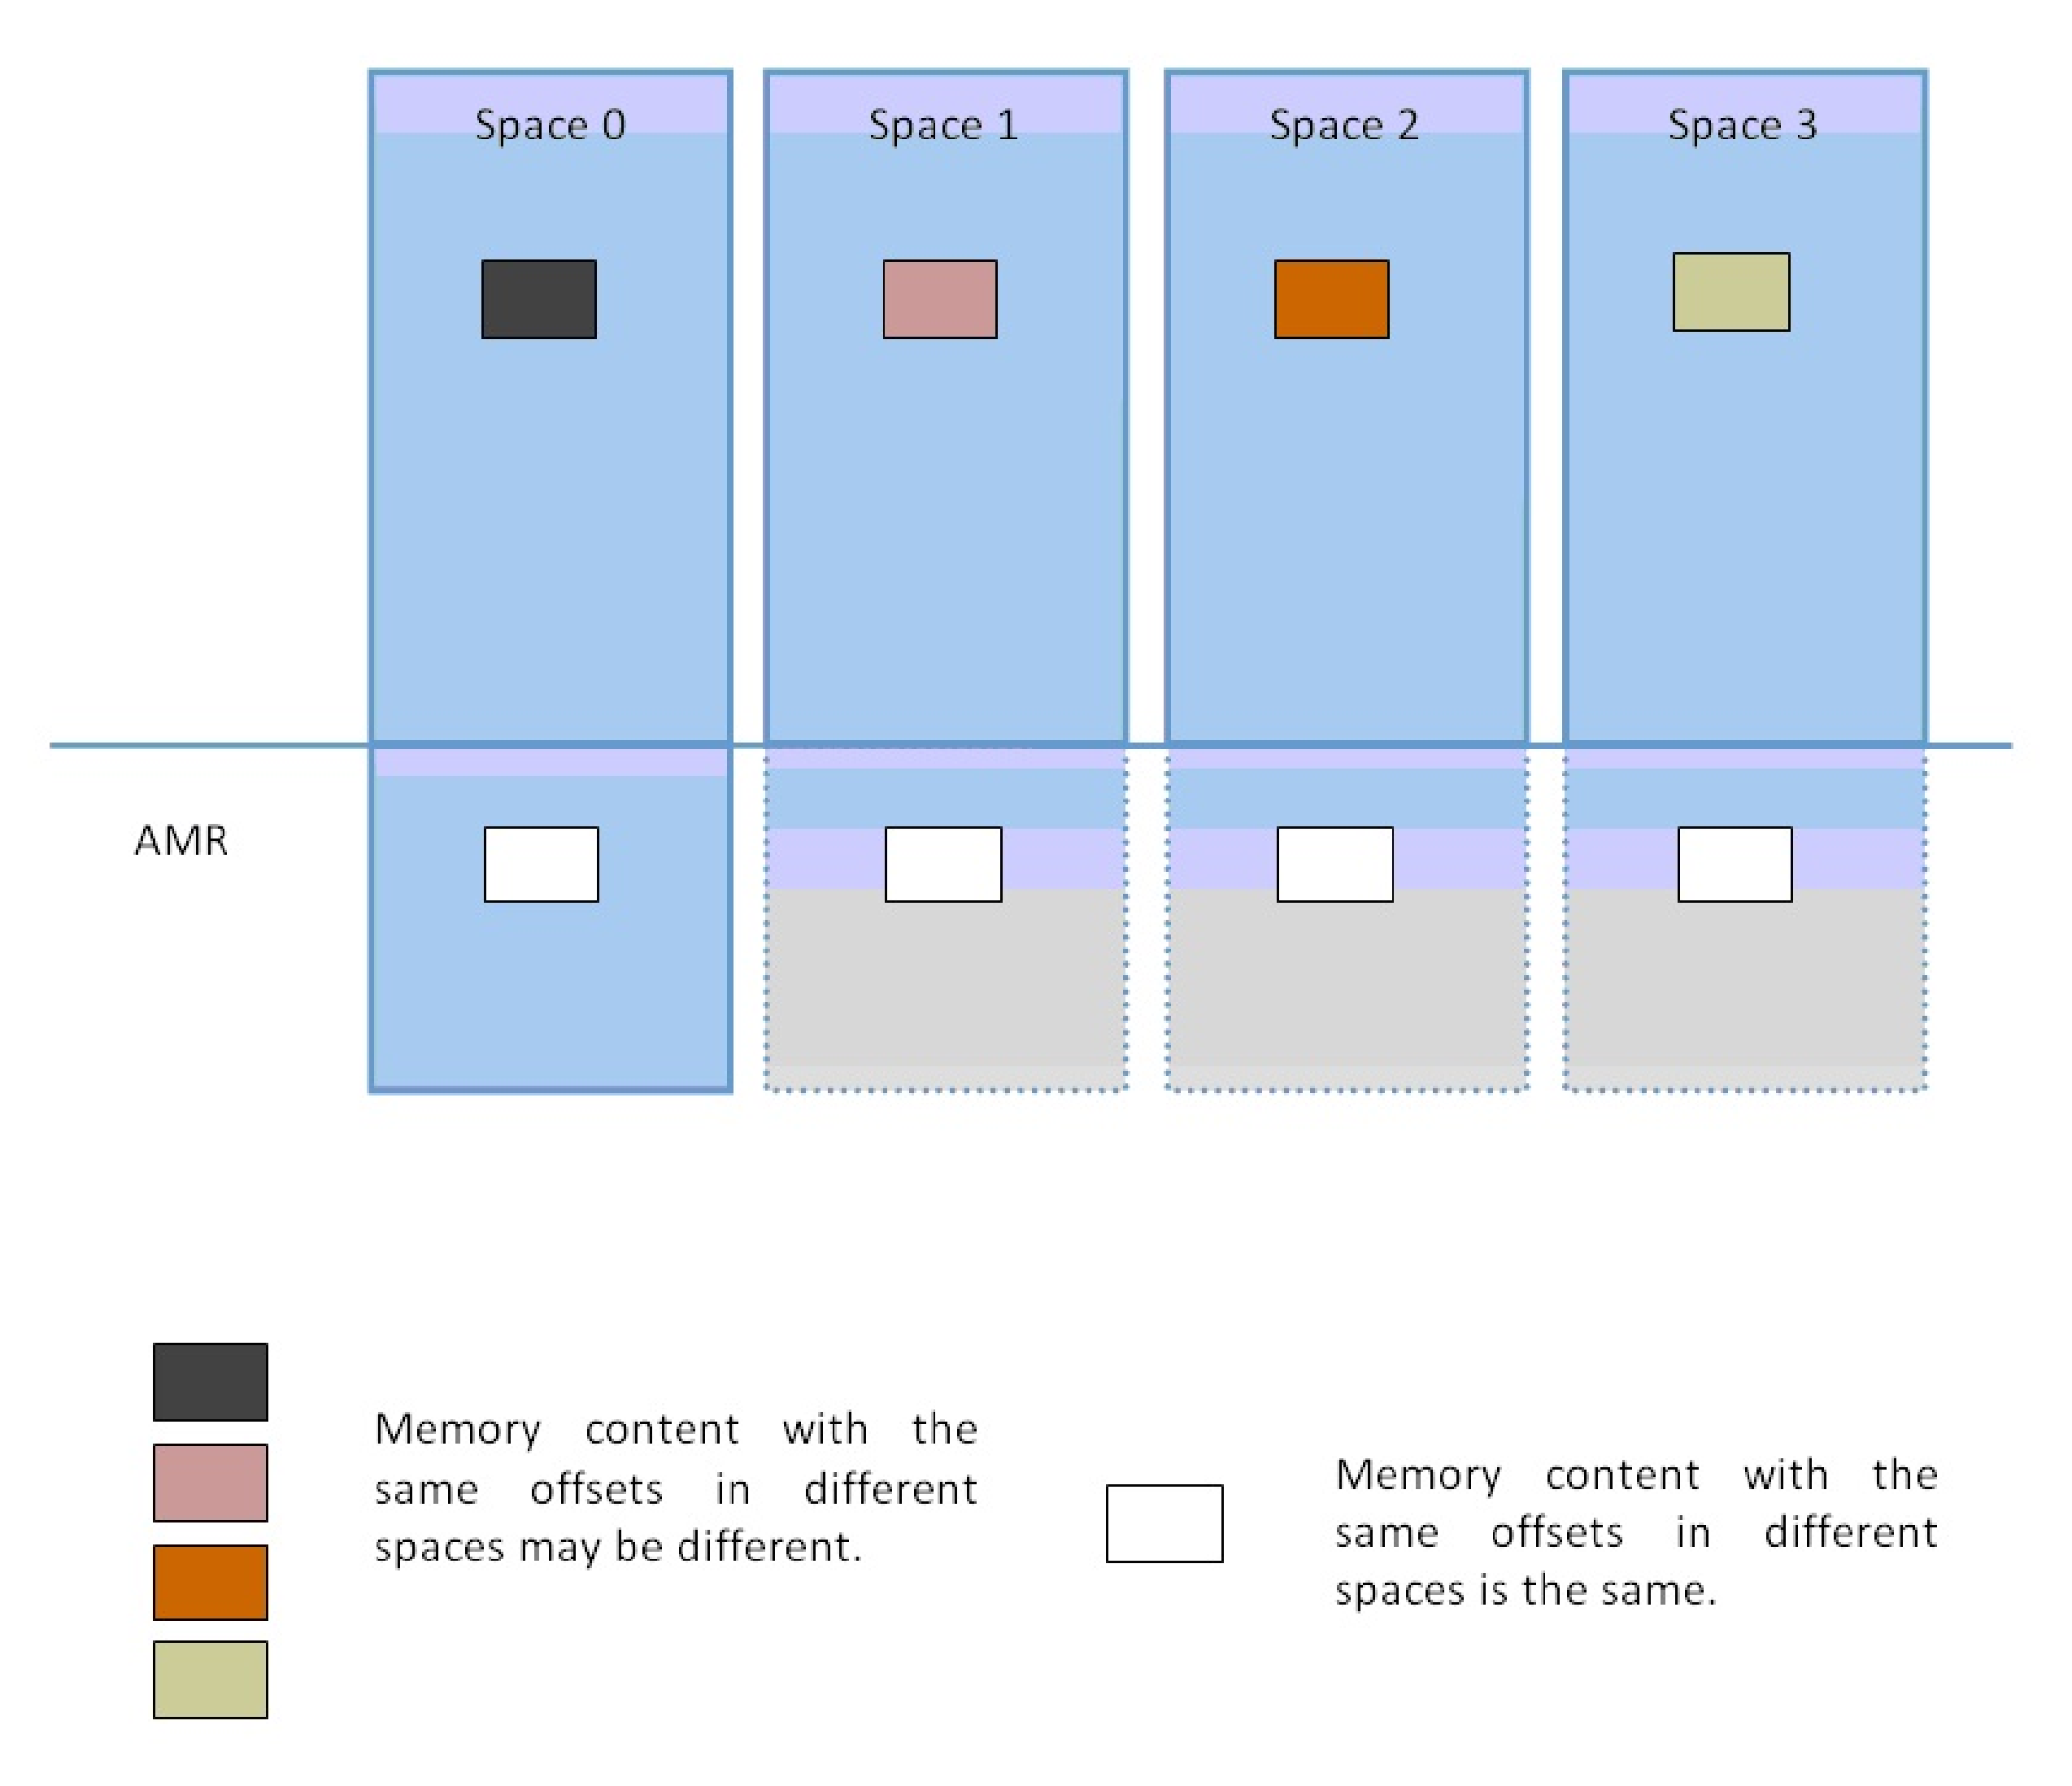
\includegraphics[width=14cm]{figure/spaces.eps}
  \caption{Spaces}
  \label{fig:c0-spaces}
\end{center}
\end{figure}

The memory layout from the view inside of one space is as in Table~\ref{table:c0-memory}.

\definecolor{webgreen}{rgb}{0,.5,0}
\begin{table}[h]
\centering
\label{table:c0-memory}
\caption{Memory layout}
\begin{tabular}{|l|l|l|}
\hline
Higher address & & L0 memory type (indicated in\\
 & & colors):\\\cline{2-2}
 & & \color{webgreen}{Heap} \\ %\cline{1-1}
 & & \color{red!20!white}{Stack} \\ %\cline{1-1}
 & & \\ \cline{2-2}
 & \colorbox{webgreen}{[Task j] Additional Heap range of (array segments)} & \\ \cline{2-2}
 & & * The locations and sizes of\\ \cline{2-2}
 & \colorbox{red!20!white}{[Task 0] Stack (grows to lower address)} & additional heap ranges may be\\\cline{2-2}
 & \colorbox{red!20!white}{...} & overlapped with other\\\cline{2-2}
 & \colorbox{red!20!white}{[Task i] Stack (grows to lower address)} & stack/heap ranges, depending on\\\cline{2-2}
 & \colorbox{red!20!white}{...} & the location of array segments\\\cline{2-2}
 & & passed in the startup parameters.\\\cline{2-2}
 & \colorbox{webgreen}{[Task i*] Additional Heap range of array segments} & \\\cline{2-2}
 & & \\\cline{2-2}
 & \colorbox{webgreen}{[Shared] Runtime Heap (grows to higher address)} & \\\cline{2-2}
 & \colorbox{webgreen}{.bss (Global variables without initial value)} & \\\cline{2-2}
 & \colorbox{webgreen}{.data (Global variables with initial values)} & \\\cline{2-2}
 & \colorbox{webgreen}{[Shared] .rodata (Read-only data)} & \\\cline{2-2}
 & \colorbox{webgreen}{[Shared] .text (Code)} & \\\cline{2-2}
 & & \\\cline{2-2}
 & L0 Internal range & \\\cline{2-2}
 & & \\\cline{2-2}
 Lower address & & \\
 & & \\\cline{2-2}
\hline
\end{tabular}
%\end{tabular*}
\end{table}

{\subsection{Program loading}}

A c0 program will be compiled into a binary in the ELF format.
At the start of the L0, the program loader will perform the following operations

\begin{itemize}
	\item Load the ELF binary from the disk
	\item Parse the ELF headers
	\item For each section of ELF. (We only use the following sections: ".text", ".data", ".rodata", ".bss". )
		\begin{itemize}
			\item Allocate the virtual memory range
			\item Copy/map the data block into the memory; note that the length of data block might be less than the memory range. Fill the rest of the space with zeros.
		\end{itemize}
	\item Create a snapshot, includes:
		\begin{itemize}
			\item Heap: all the memory ranges of the ELF sections in memory
			\item Initial dynamic heap with fixed size (e.g.1GB?, but we don't need to allocate memory pages now)
			\item Fixed size (e.g. 64KB?) stack
		\end{itemize}
	\item Start a new task with the entry point and the created snapshot.
\end{itemize}
The memory layout is illustrated in Fig.~\ref{fig:c0-elf}[1].\\
\begin{figure}[htbp]
\begin{center}
  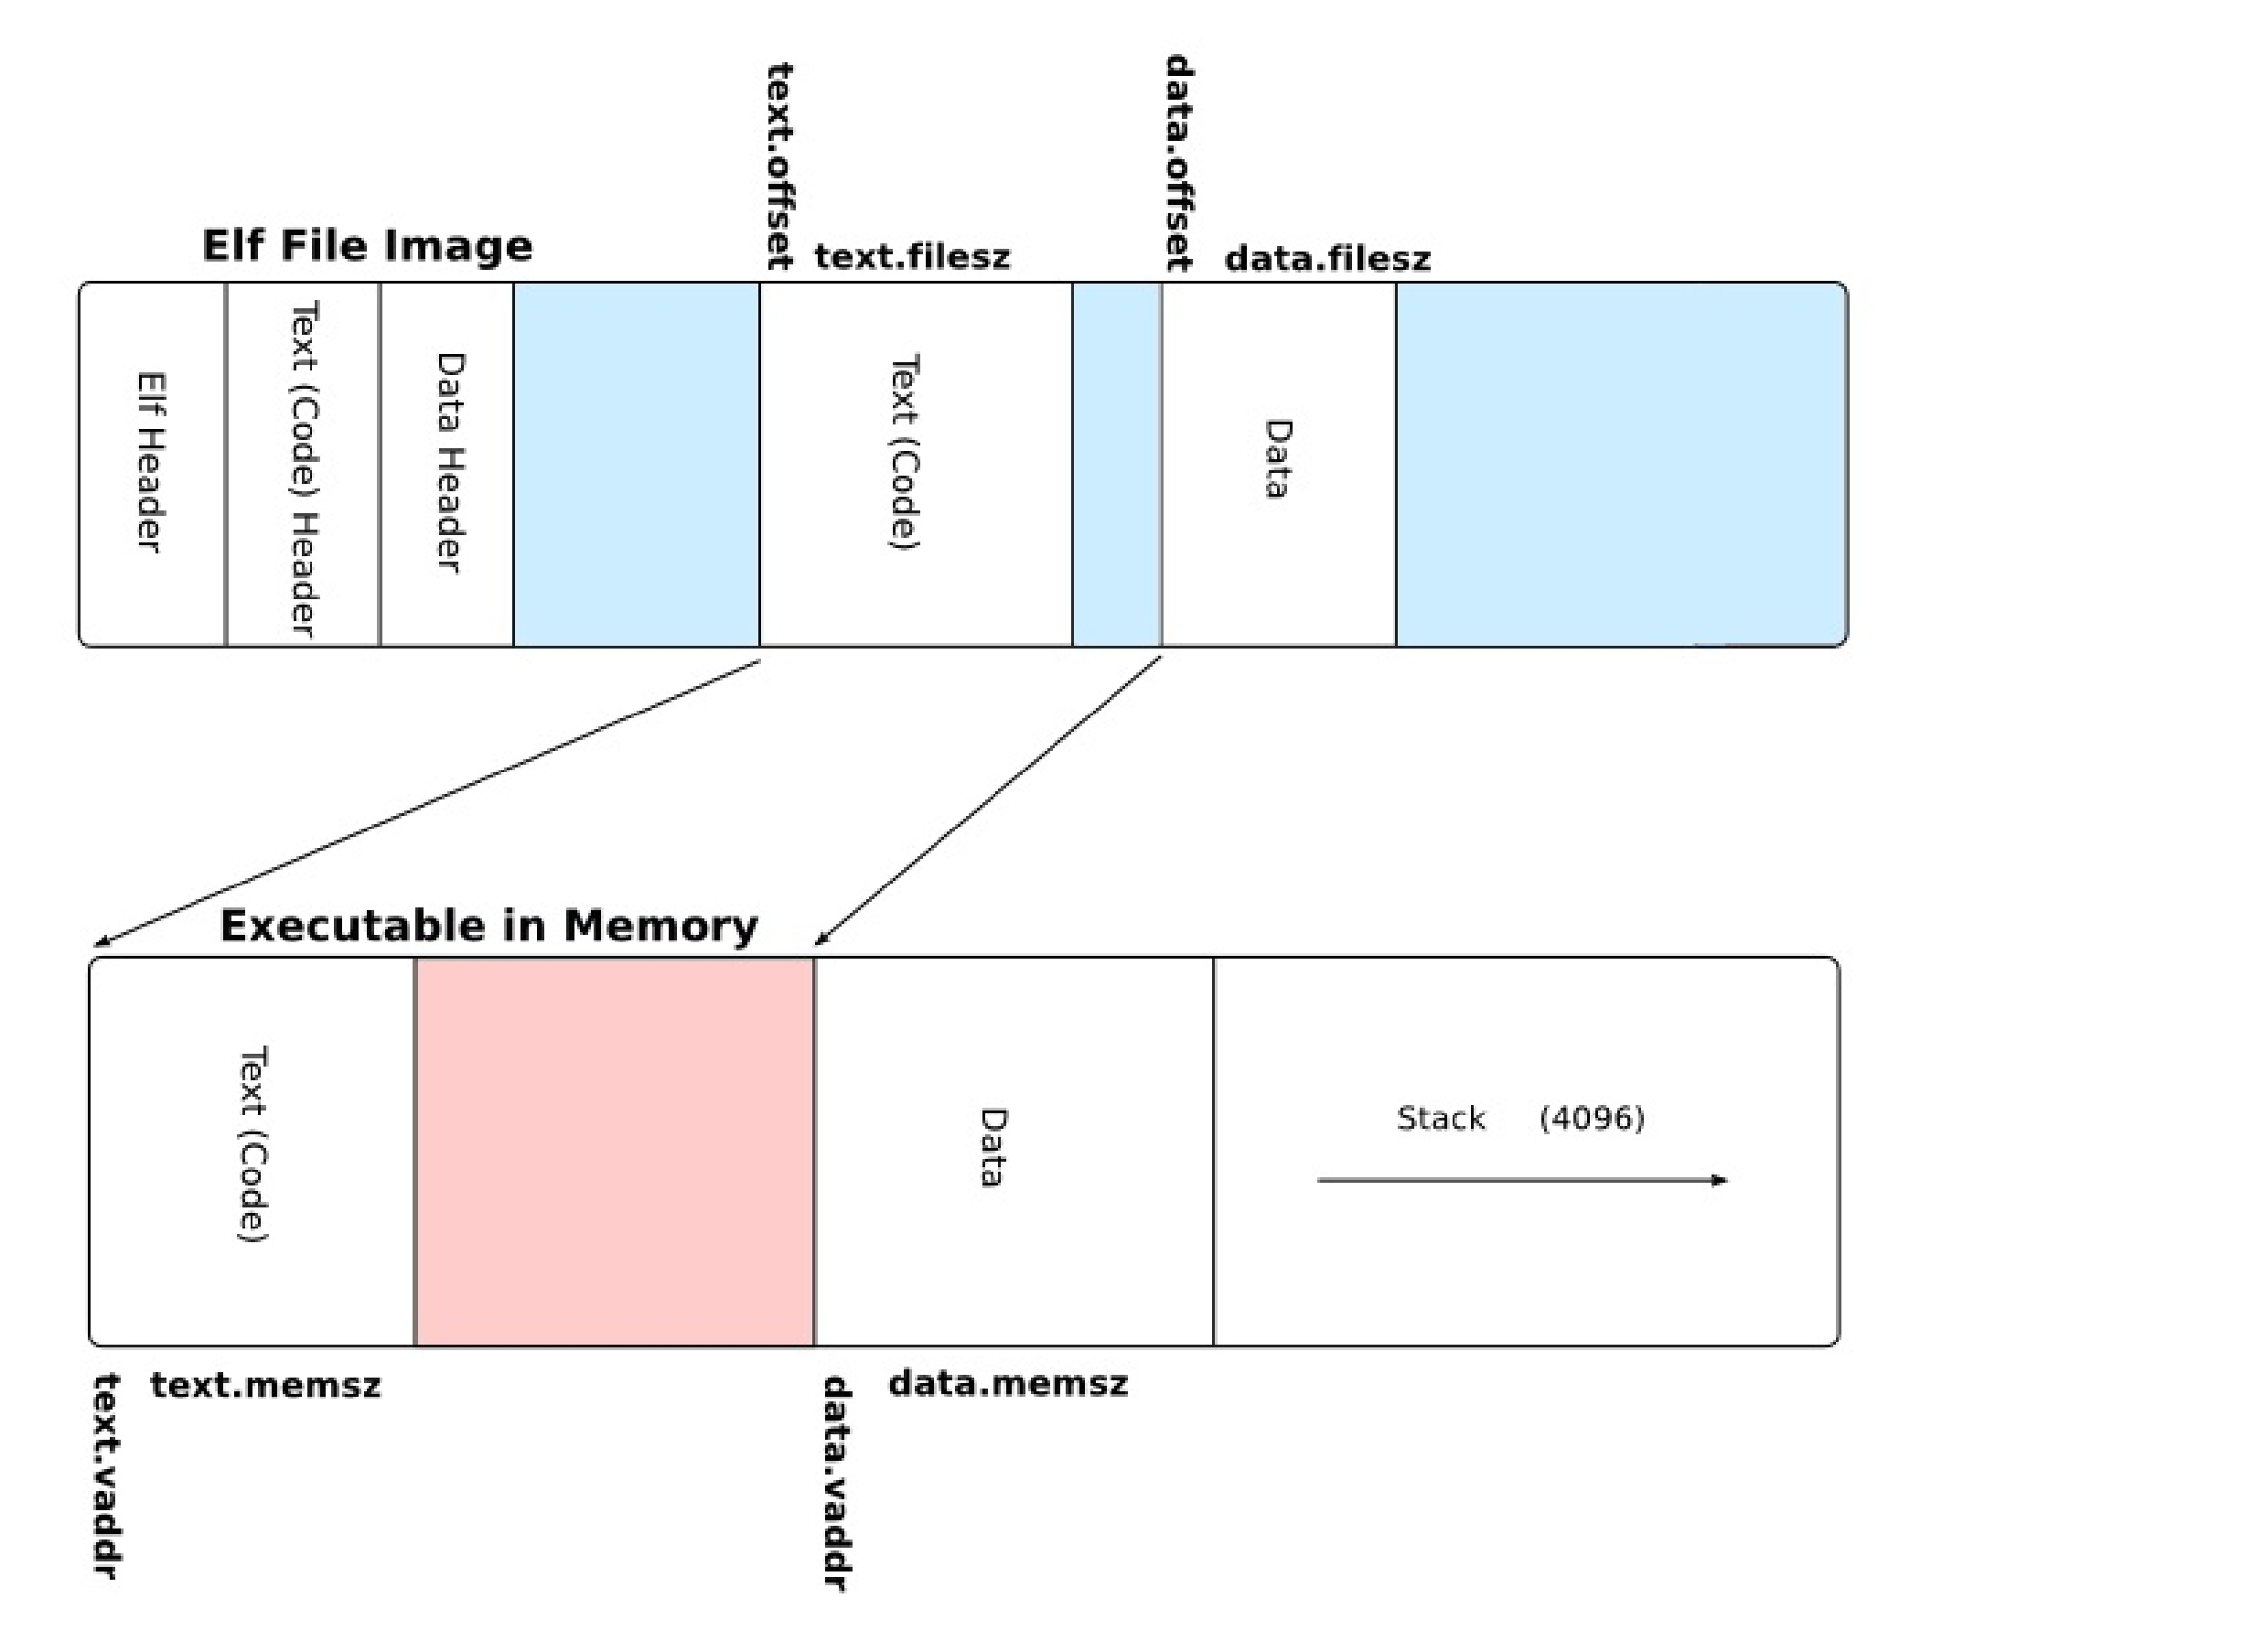
\includegraphics[width=14cm]{figure/elf.eps}
  \caption{ELF file loading}
  \label{fig:c0-elf}
\end{center}
\end{figure}

\line(1, 0){450}\\

Update History\\

\begin{itemize}
	\item Originally written by Xiang Gao.
	\item May. 8, 2013. Add space for the task statement. - zma
	\item Feb. 5, 2014. Revise this document. - Weiwei Jia
	\item Feb. 18, 2014. Revise this document. - Zhiqiang ma, Weiwei Jia
	\item Feb. 24, 2014. Corrected several typos and improved writings of several places. - Zhiqiang Ma
	\item Feb. 26, 2014. Add standalone-related stuff for keywords and a section to introduce it. - zma
	\item Feb. 28, 2014. Revisions from lingu; add a figure illustrating the spaces. - zma
	\item Feb. 28, 2014. Mark that `double` are supported; `int` is buggy yet. - zma
	\item Mar. 20, 2014. Mark bitwise AND, OR and XOR (\&, |, {\char`\^}) that is supported. Fix several strange names. - zma
	\item Apr. 3, 2014. Translate C0 doc into Latex version. - Weiwei Jia.
    \item Apr. 6, 2014. Resize the figure 1, 2 and table 4 and make them closer to corresponding descriptions.
    \item Apr. 29, 2014. Add the ``differene between commit/abort and commitd/abortd''. - zma
    \item May. 16, 2014. Refined writing. - zma
\end{itemize}

\color{black}{\line(1, 0){450}}\\

[1] http://wiki.osdev.org/ELF

\end{document}
